Nei capitolo precedenti sono stati introdotti i concetti teorici e operativi necessari alla realizzazione del progetto. In particolare nel Capitolo 1 sono stati descritti i fondamenti geometrici e matematici alla base della rappresentazione e manipolazione di oggetti 3D, mostrando come mesh, trasformazioni e sistemi di coordinate permettano di modellare e controllare il movimento nello spazio tridimensionale. Nel capitolo 2, invece, è stato analizzata la pipeline di animazione attrraverso tool e software specifici, soffermandosi sul rigging, sullo skinning e sulle tecniche di acquisizione e trasferimento del movimento tramite sistemi di motion capture.

In questo capitolo tali conoscenze vengono applicate nella costruzione del workflow sviluppato per la presente tesi. L'obbiettivo è automatizzare il trasferimento di animazioni umanoidi verso modelli non convenzionati, riducendo l'intervento manuale e rendendo il processo più efficente e scalabile. Verranno quindi illustrate le fasi operative che compongono la pipeline: a partire dell'importazione e test delle animazioni umanoidi, passando per la generazione automatica dello scheletro e l'assegnazione dei pesi alla mesh, fino al retargeting dell'animazione e all'integrazione finale in Unity. Ogni sezione descriverà sia gli strumenti utilizzati sia gli script utilizzati, mettendo in evidenza le scelte progettuali adottate e i risultati ottenuti.

\section{Importazione dei modelli umanoidi}

L'importazione del modello 3D rappresenta il primo passo fondamentale nel processo di animazione di un personaggio umanoide. Affinchè un modello possa essere animato correttamente, esso deve essere dotato di una struttura scheletrica interna (rig) che consenta la manipolazione delle articolazioni e la deformazione della mesh. La qualità e la correttezza dei rig influenzano direttamente la fluidità e la naturaleza dei movimenti, rendendo questa fase cruciale per l'intera pipeline di animazione.

In ambito di sviluppo videoludico e applicazioni interattive, i modelli umanoidi vengono generalmente importati da librerie esterne o realizzati tramite software di modellazione 3D. Tuttavia , è necessario assicurarsi che il formato del file sia compatibile con il motore di sviluppo utilizzato: il formato FBX è il più diffuso in quanto permette di importare non solo la geometria del modello, ma anche la rig e, se presenti, le animazioni predefinite.

L'obiettivo di questa sezione è quindi descrivere i principali formati di file utilizzati, le fonti più comuni per l'acquisizione di modelli umanoidi e le impostazioni necessarie per garantire una corretta integrazione del personaggio all'interno dell'ambiente Unity.

\subsection{Tipologie di modelli (Mixamo, Unity Asset Store)}

Piattaforme come Mixamo e Unity Asset Store mettono a disposizioni personaggi già riggati, riducendo significativamente i tempi di preparazione e permettendo di concentrarsi sulla fase di animazione.

Mixamo, un servizio offerto da Adobe, mette a disposizione una libreria molto vasta di personaggi 3D completi di scheletro. La peculiarità di Mixamo risiede nel sistema di auto-rigging, che permette di applicare automaticamente uno scheletro umanoide a un modello caricato dall'utente.
L'Unity Asset Store, invece, è un marketplace integrato nel motore Unity, che offre modelli 3D sviluppati da artisti e studi professionisti. I modelli presenti nello store variano notevolmente in termini di complessità, qualità delle texture, dettaglio del rig e presenza o meno di animazioni incluse.

\begin{figure}[h]
\begin{center}
     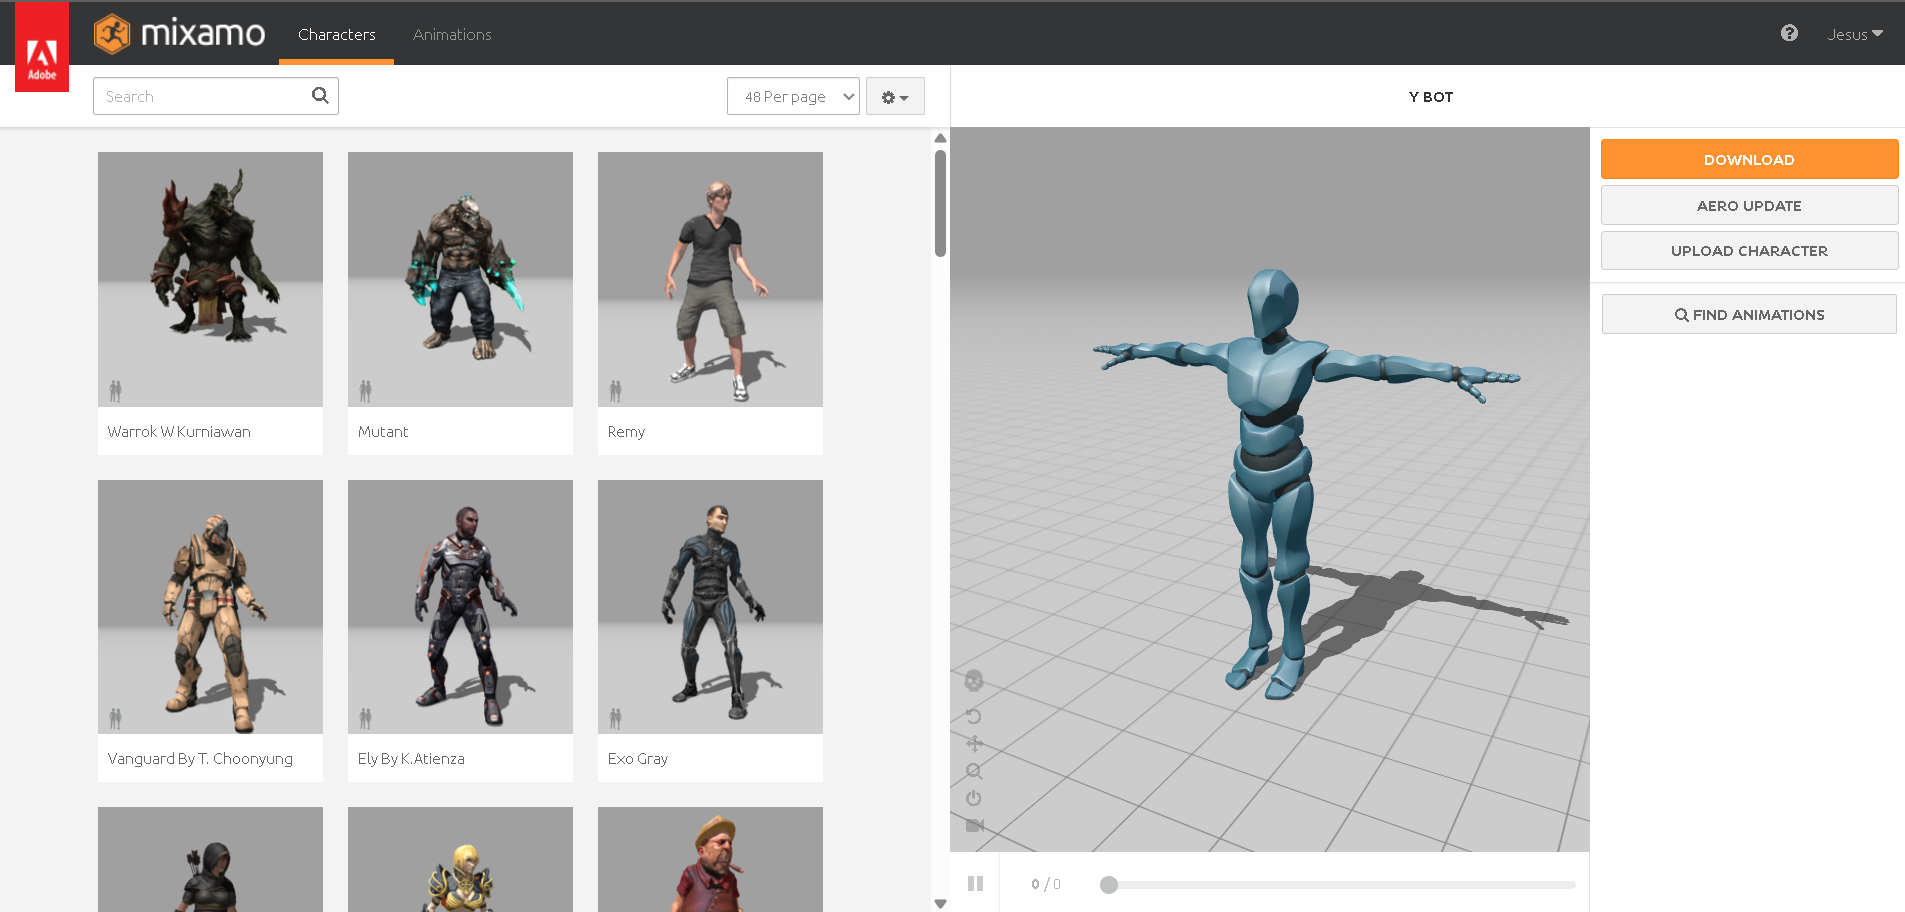
\includegraphics[width=10cm]{figure/mixamo2.png}
     \caption{Software Mixamo}
\end{center}
\end{figure}

\subsection{Formati supportati (FBX, OBJ)}

Nella fase di importazione dei modelli umanoidi in Unity, il formato del file riveste un ruolo fondamentale, poichè determina quali informazioni saranno effettivamente trasferite all'interno del progetto. I due formati più utilizzati in questo contesto sono FBX  e OBJ, ciascuno caratterizzato da specifiche funzionalità e limiti.

Il formato FBX (Filmbox) è considerato lo standard nell'ambito dell'animazione 3D e della produzione videoludica. Oltre alla mesh del modello, l'FBX è in grado di contenere al suo interno la struttura scheletrica (rig), le animazioni associate, le informazioni sui materiali e le texture. Grazie a queste caratteristiche, l'FBX permette di trasferire un modello completo direttamente da software di modellazione come Blender, Maya o 3ds Max a Unity, mantenendo intatta la gerarchia delle ossa e la corretta disposizione delle animazioni.
Al contrario, il formato OBJ è molto più semplice e limitato. Esso rappresenta esclusivamente la geometria della mesh, senza contenere rig nè animazioni. Questo lo rende adatto per modelli statici o come base per successivi processi di rigging ed animazione, ma non per una importazione diretta di personaggi già animabili.

In questa fase, l'obbiettivo principale è garantire che il modello umanoide sia pronto per ricevere animazioni, senza intervenire ancora su rigging, skinning o retargeting automatico, che saranno approfonditi nei capitoli successivi.

\section{Applicazione di animazioni predefinite}

Una volta importato il modello umanoide nell'ambiente di sviluppo, è possibile procedere con l'applicazione delle animazioni. L'utilizzo di animazioni predefinite consente di ridurre notevolmente i tempi di produzione, evitando la necessità di creare manualmente i movimenti tramite tecniche di keyframing o sistemi di motion capture. Le animazioni predefinite sono generalmente organizzate in librerie, come quelle messe a disposizione da Mixamo, dall'Unity Asset Store o da altri archivi professionali di motion data.

Unity facilita l'integrazione delle animazioni attraverso il sistema di configurazione del rig Humanoid, che permette di adattare automaticamente le animazioni anche tra modelli differenti. Ciò significa che una stessa animazione , se correttamente configurata, può essere riutilizzata su più personaggi, a condizione che dispongano di una struttura scheletrica compatibile.

\subsection{Animazioni di base: camminata, corsa, salti}

Le animazione considerate "base" sono quelle che descrivono le azioni fondamentali del movimento umano. Tra le più comuni si trovano:

\begin{itemize}
    \item \textbf{Idle}: posizione di riposo del personaggio
    \item \textbf{Walk cycle}: ciclo completo di camminata.
    \item \textbf{Run cycle}: ciclo di corsa, caratterizzato da maggiore ampiezza e ritmo del movimento.
    \item \textbf{Jump}: animazione di salto, tipicamente suddivisa in tre fasi (preparazione, fase aerea e atterraggio).
\end{itemize}

\begin{figure}[H]
\centering
\begin{subfigure}{0.48\textwidth}
  \centering
  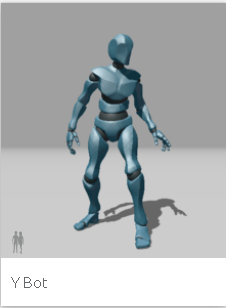
\includegraphics[height=4cm, keepaspectratio]{figure/Y-bot.png}
  \caption{Y-bot}
\end{subfigure}\hfill
\begin{subfigure}{0.48\textwidth}
  \centering
  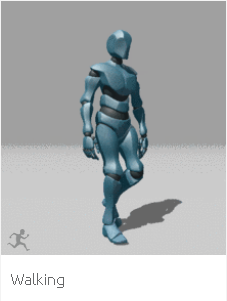
\includegraphics[height=4cm, keepaspectratio]{figure/walk.png}
  \caption{walking}
\end{subfigure}

\vspace{0.6em}

\begin{subfigure}{0.48\textwidth}
  \centering
  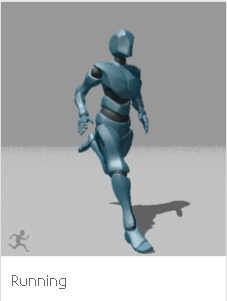
\includegraphics[height=4cm, keepaspectratio]{figure/run.png}
  \caption{Running}
\end{subfigure}\hfill
\begin{subfigure}{0.48\textwidth}
  \centering
  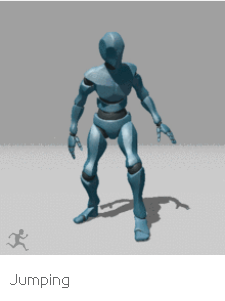
\includegraphics[height=4cm, keepaspectratio]{figure/jump.png}
  \caption{Jumping}
\end{subfigure}
\caption{Animazioni base.}
\end{figure}



Queste animazioni costituiscono la base per il controllo del personaggio in un ambiente interattivo, come un videogioco o una simulazione. Durante l'importazione delle clip, Unity consente di analizzare e modificare le proprietà delle animazioni, come la ripetizione ciclica (loop), la sincronizzazione dei piedi o la gestione del movimento della radice (root motion), migliorando la fluidità e la naturalezza del risultato finale.

\subsection{Librerie di animazioni e compatibilità con i rig}

Le librerie di animazioni predefinite possono variare per stile, complessità e struttura scheletrica di supporto. Quando si utilizza una libreria, è importante assicurarsi che l'animazione sia compatibile con il rig del modello. Unity supporta questa operazione tramite il sistema di retargeting Humanoid, che consente di adattare le animazioni a scheletri differenti mantenendo la corretta corrispondenza anatomica tra le ossa.

Se il modello e l'animazione sono entrambi configurati come Humanoid, Unity può applicare automaticamente l'animazione anche se proviene da un personaggio con proporzioni diverse. In caso contrario (ad esempio con rig personalizzati o non umani), è necessario intervenire manualmente sulla mappatura delle ossa o utilizzare strumenti esterni di rigging e editing dell'animazione.

In questo modo, l'adozione delle libreria di animazioni predefinite consente di ottenere risultati rapidi e coerenti, permettendo di concentrare gli sforzi creativi sulla logica di interazione e sul comportamento del personaggio piuttosto che sulla fasi dettagliate di creazione del movimento.

\section{Pipeline di integrazione animazione}

L'integrazione delle animazioni all'interno di Unity si basa su una pipeline strutturata che consente di importare correttamente il modello umanoide, configurarne il rig, associare le clip di animazione e gestirne la transizione durante l'esecuzione dell'applicazione. Tale processo assume un ruolo centrale nello sviluppo di personaggi interattivi, porchè definisce il modo in cui le animazioni vengono interpretate e riprodotte dal motore grafico. La pipeline può essere suddivisa in diverse fasi consecutive, che vanno dall'esportazione del modello da un software esterno fino alla definizione della logica di controllo dei movimenti attraverso l'\textbf{Animator Controller}(Figura ~\ref{fig:cont}).

\begin{figure}[h]
\begin{center}
     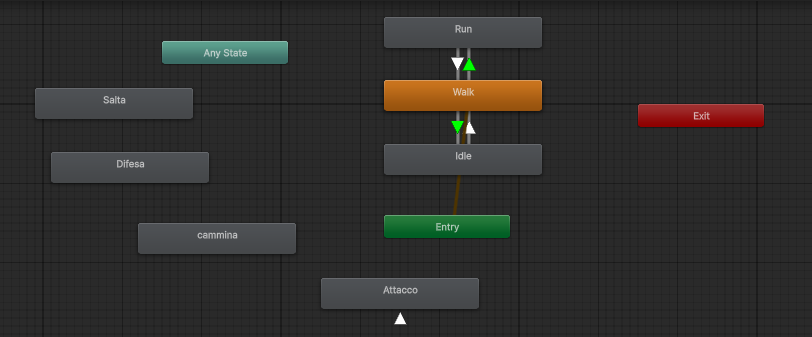
\includegraphics[width=12cm]{figure/controller.png}
     \caption{Animation Controller con diverse animazioni}
     \label{fig:cont}
\end{center}
\end{figure}

\subsection{Esportazione e importazione del modello (FBX -> Unity)}

Il primo passaggio consiste nell'esportazione del modello e delle relative animazioni da un software di modellazione 3D o da un piattaforma di librerie come Mixamo. Il formato maggiormente utilizzato è FBX, in quanto consente di preservare la struttura gerarchica dello scheletro, le pesature dei vertici e le curve di animazione associate.

Una volta inserito il file FBX all'interno del progetto Unity, il motore provvede alla sua conversione automatica nel formato interno. A questo punto, l'utente può accedere al pannello delle \textbf{Import Settings} (Figura~\ref{fig:confi}), che consente di definire la tipologia di rig tramite l'impostazione \textbf{Humanoid}, garantendo così la compatibilità con il sistema di retargeting del motore. Inoltre, nella sezione Animation, è possibile separare le clip contenute nel file, attivarne il loop, normalizzarne la durata o abilitare l'opzione \textbf{Root Motion} (Figura~\ref{fig:inspe}), che influenzerà la gestione del movimento nello spazio tridimensionale.

\begin{figure}[h]
\begin{center}
     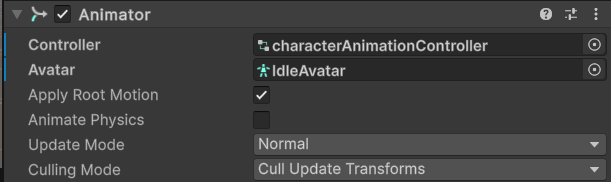
\includegraphics[width=10cm]{figure/inspe.png}
     \caption{Proprietà di un oggetto selezionato}
     \label{fig:inspe}
\end{center}
\end{figure}

\textbf{Proprietà dell'oggetto selezionato}
\begin{enumerate}
    \item \textbf{Controller}: il Animation Controller collegatto all'oggetto.
    \item \textbf{Avatar}: l'Avatar per questo personaggio (se l'Animatore viene usato per animare un personaggio umanoide).
    \item \textbf{Apply Root Motion}: seleziona se controllare la posizione e la rotazione del personaggio dall'animazione stessa o dallo script.
    \item \textbf{Update Mode}: questo ti permette di selezionare quando l'Animator aggiorna e quale scala temporale deve utilizzare
    \begin{enumerate}
        \item \textbf{Normale}: L'Animator viene aggiornato in sincronia con la chiamata Update, e la velocità dell'animatore corrisponde a quella attuale. Se la scala temporale è rallentata, le animazioni rallenteranno per adattarsi.
        \item \textbf{Animate Physics}: L'animatore viene aggiornato in sincronia con al chiamata FixedUpdate (cioè in perfetta sincronia con il sistema fisico). Dovresti usare questa modalità se stai animando il movimento di oggetti con interazioni fisiche, come i personaggi che possono spingere oggetti rigidbody.
        \item \textbf{Unscaled Time}: L'animatore viene aggiornato in sincronia con la chiamata Update, ma la velocità dell'animatore ignora la scala temporale attuale e anima comunque al 100\% della velocità. Questo è utile per animare un sistema GUI a velocità normale usando scale temporali modificate per effetti speciali o per mettere in pausa il gameplay.
    \end{enumerate}
    \item \textbf{Culling Mode}: la modalita culling puoi scegliere per le animazioni.
    \begin{enumerate}
        \item \textbf{Always animate}: animare sempre, non fare culling anche fuori campo.
        \item \textbf{Cull Update Transforms}: Retarget, IK e scrittura delle trasformazioni sono disabilitate quando i renderer non sono visibili.
        \item \textbf{Cull Completely}: l'animazione è completamente disabilitata quando i renderer non sono visibili.
    \end{enumerate}
    
\end{enumerate}

\subsection{Animator Controller e gestione degli stati di animazione}

Una volta importate le animazioni, è necessario definire le modalità con cui il personaggio passerà da un movimento all'altro durante l'esecuzione. Unity utilizza a tal fine l'\textbf{Animator Controller}, una macchina a stati finiti che rappresenta le diverse animazioni come nodi collegati da transizioni. Ogni transizione può essere controllata tramite parametri (booleani, interi, float o trigger), modificabili a runtime tramite script o input dell'utente.

Questo approccio consente di gestire in modo modulare e scalabile sequenze complesse di movimenti, come la transizione fluida tra camminata e corsa o la sincronizzazione tra salto e aterraggio. Inoltre, Unity mette a disposizione strumenti avanzati come i \textbf{Blend Trees}, che permettono di interpolare più animazioni in funzione di un parametro continuo (ad esempio la velocità), garatendo una maggiore naturaleza nell'esecuzione delle animazione di locomozione.

Un'architettura dell'Animator Controller ben progettata consente quindi una maggiore flessibilità, favorisce il riutilizzo delle animazioni e semplifica l'eventuale estensione futura del sistema di controllo del personaggio.

\section{Gestione dei modelli animati}

Nel progetto sviluppato, la gestione del modello umanoide risulta semplificata dal fatto che il personaggio utilizzato era già dotato di rig completo e di corretta associazione tra mesh e scheletro. Pertanto, non è stato necessario intervenire sul processo di \textit{skinning} o sulla definizione dei pesi dei vertici, operazioni che normalmente richiederebbero l'utilizzo del software di rigging come Blender o Maya. Unity ha riconosciuto automaticamente la struttura scheletrica del modello e ha provveduto  a configurarla secondo il sistema \textbf{Humanoid}, permettendo così di applicare animazioni predefinite sensaz ulteriore modifiche.

La riproduzione delle animazioni è stata gestita tramite l'\textbf{Animator Controller}, che ha permesso di definire e controllare le transizioni tra i diversi stati animati, come ad esempio il passaggio da idle a camminata o corsa. Poiché il modello era già predisposto per l'utilizzo delle animazioni umane standard, l'applicazione delle clip è avvenuta in modo diretto, senza la necessità di operazioni di retargeting manuale o adattamento delle pose.

Queste condizione ha semplificato la pipeline di animazione, rendendo il processo più rapido ed efficiente. Rispetto a modelli non organici o non riggati, dove sarebbe necessario costruire uno scheletro artificiale e definire le influenze delle ossa sulla superficie della mesh, nel caso degli umanoidi la struttura preesistente consente un'applicazione immediate e riutilizzabile delle animazioni.

In sintesi, l'utilizzo di un modello già riggato e compatibile con il sistema Humanoid di Unity ha permesso di concentrarsi esclusivamente sulla gestione dell'Animator Controller e delle animazioni, semplificando notevolmente il flusso di lavoro rispetto a oggetti non animati o con rig personalizzato.


\section{Retargeting su umanoidi}

Il retargeting è una procedura che consente di applicare la stessa animazione a modelli diversi, purché condividano una struttura scheletrica compatibile. Nel caso dei personaggi umanoidi, Unity dispone di un sistema di retargeting integrato basato sullo standard \textbf{Humanoid Rig}, che permette di trasferire animazioni tra modelli diferenti mantenendo la coerenza dei movimenti. Questo processo risulta particolamente utile quando si utilizzano librerie di animazioni esterne, come quelle fornite da Mixamo, oppure quando si integrano personaggi provenienti da diverse fonti di modellazione 3D (tipo MoveAI).  

\subsection{Concetto di retargeting tra rig simili}

Il sistema Humanoid di Unity definisce una mappatura standard delle principali articolazioni del corpo (test, colonna vertebrale, braccia, gambe, mani). Quando il modello viene importato e configurato come Humanoid, Unity riconosce automaticamente l'equivalente dello scheletro intero e consente di utilizzare animazioni create per altri personaggi umanoidi.
In termini pratici, ciò significa che un'animazione di camminata può essere applicata a qualsiasi modello umanoide senza la necessità di ricreare manualmente il movimento.

\subsection{Metodi automatici semplificati (solo per personaggi umanoidi)}

Unity gestisce il retargeting in modo quasi completamente automatico. È sufficiente:

\begin{enumerate}
    \item Importare il modello come \textbf{Humanoid Rig}
    \item Associare una clip di animazione proveniente da un'altra sorgente
    \item Applicarla tramite l'\textbf{Animator Controller}
\end{enumerate}

Grazie a questa funzione, è possibile riutilizzare un'ampia gamma di animazioni già presenti nelle librerie, riducendo significativamente il tempo richiesto per la produzione di movimenti realistici.

\begin{figure}[H]
\begin{center}
     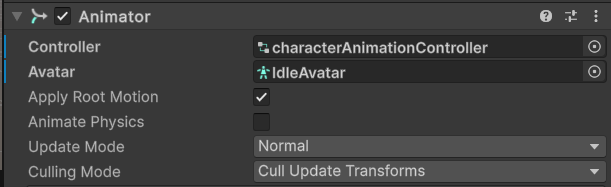
\includegraphics[width=12cm]{figure/retar.png}
     \caption{Applicazione animazioni create per un modello}
     \label{fig:retar}
\end{center}
\end{figure}

\subsection{Limitazioni rispetto a oggetti non organici}

Il retargeting automatico presente nei software moderni (es. Blender, Unity, MotionBlender) si basa quasi sempre su un modello \textbf{umanoide standardizzato}, caratterizzato da un struttura scheletrica prevedibile (colonna vertebrale, braccia, gambe, testa) e da vincoli cinematici tipici dell'anatomia umana.

Quando l'oggetto da animare \textbf{non possiede caratteristiche antropomorfe}, questa pipeline non risulta applicabile o perde grande parte della sua efficacia. Oltre ai casi già citati (creature non umanoidi, oggetti meccanici, strutture articolate atipiche), esistono varie categorie problematiche:

Perche il retargeting automatico fallisce
\begin{enumerate}
    \item \textbf{Assenza di una corrispondenza diretta tra giunti}: 
    I sistemi umanoide prevedono un mapping "uno-a-uno" tra ossa equivalenti (Hips -> Hips, Spine -> Spine, ecc.).
    
    \item \textbf{Topologia scheletrica non compatibile}
    Creature multipedali, insetti, robot o oggetti inventati presentano:
    \begin{itemize}
        \item più arti o meno arti
        \item articolazioni non lineari (segmenti meccanici, giunti cilindrici, pistoni, tentacoli)
        \item strutture non gerarchiche
    \end{itemize}
    \item \textbf{Range di movimento non umano}
    Gli algoritmi umanoidi assumono vincoli cinematici:
    \begin{itemize}
        \item cavallo pelvico
        \item limitazioni di abduzione/adduzione
        \item articolazioni sferiche/hinge
            Oggeti artificiali possono violare tutti questi limiti (rotazione 360 gradi, assi multipli, traslazioni)
    \end{itemize}
    \item \textbf{Root motion non universale}
    Il movimento radie negli umanoidi è centrato su Hips/Pelvis. In un robot o in una creatura aliena, la "root" può essere ovunque.
\end{enumerate}


